\clearpage
\section{Abstract}
\label{sec:org4433b66}
This thesis has so far explored the measurement and modeling of movement of (terrestrially) locomoting animals.
A topic which remains to be discussed is the \emph{cause} of that movement.
The segments of animal limbs can be modeled as rigid bodies, each of which has a specific momentum.
Momentum is a conservative quantity, i.e. it changes due to energy transfer with its surrounding.
The retrospective inference of reasons for momentum change is often labeled ``inverse dynamics''.

The field of (inverse) dynamics is subject to various conventions and some methodological flexibility.
The purpose of this chapter is to set the table and clarify conventions used further on in this thesis.
The physical fundamentals and general algorithms applied in inverse dynamic calculations are presented, as well as elegant mathematical tools to implement them (wrenches, quaternions).
To illustrate the basic principles of physics which come to play in this chapter, a hypothetical collision experiment is discussed.
It turns out that, whereas most quantities in inverse dynamic calculations can be accurately measured, the inertial properties of segments are the Achilles heel of accurate dynamic modeling.



\begin{figure}[p]
\centering
\includegraphics[width=12cm]{./figures/slamming_door.pdf}
\caption{\label{fig:slamming}\textbf{A hypothetical, scientific experiment} to illustrate dynamic modeling (see text). Upper left: experimenter setting a door in motion. Lower right: subject running towards the experimental setup. \(\vec{P}\): hinge point/axis of the door, \(\vec{v}\): velocity of the subject, \(\dot\theta = \frac{d\theta}{dt}\): angular velocity of the door, \(\vec{F}\): force applied to the door by the experimenter.}
\end{figure}


\FloatBarrier\clearpage
\section{Introduction}
\label{sec:orgbb91032}
\subsection{A Momentum Experiment}
\label{sec:orgc2df572}
``Slamming a door in someone's face'' is not a friendly thing to do.
Yet ``friendliness'' is not a scientific category, and thus we must consider this as a purely physical process (Fig. \ref{fig:slamming}).
If a person in question is running at constant velocity (which we could quantify using Fourier methods and probabilistic modeling, see before), the unexpected appearance of an obstacle will certainly force the subject to change trajectory.
If the unfortunate subject is unable to adjust on time, physicists would call this a ``collision experiment''.
In most probable cases the impact will thus \textbf{change the subject's momentum}.
Momentum quantifies the linear and angular movement of a body.
The non-sliding door itself, set up on a hinge (point \(\vec{P}\) in Fig. \ref{fig:slamming}), will gain rotational momentum through the act of slamming, performed by an experimenter.
In the collision case, the subject might (i) decelerate but proceed, (ii) come to a hold, or (iii) ungently bounce backwards from the elastic collision.
The door will thus transfer momentum to the subject, thereby ultimately canceling out (part of) the momentum of the person if the impact is approximately equal in magnitude, but opposite in direction, of the running.
Trained experimenters might even succeed in (iv) transferring angular momentum to the surprised subject, generating a spin (though attention must be paid to whether that spin is partially caused by an evasive motor response of the subject).
All these possible outcomes are manifestation of the \textbf{conservation of energy and momentum}, which I will explore \chng{on the metaphor of a} hypothetical door slamming experiment.
Due to the numerous involved variables, it is not clear \emph{a priori} how exactly a subject will be hit, and what the exact consequences of the collision are.
Predicting the outcome of such scientific experiments is enabled by a major field of biomechanics, which is called \textbf{dynamic modeling}.
\subsection{Kinematics and Kinetics}
\label{sec:org1791728}
In the next chapter (Ch. \ref{cpt:inertials}), I will discuss a specific contribution to dynamic modeling, namely the extraction of inertial properties from CT scans.
This chapter serves to illustrate the overall context and to establish the connection with the previous topics of this thesis.
It answers the question of the relevance of CT-based inertial property quantification, by providing a superficial overview of the dynamic modeling technique.


Until this point, this thesis focused on methodological development in terms of measuring, modeling and predicting \emph{kinematics}.
With Fourier-based methods and probabilistic models in place, one can
  (i) quantify measured kinematics, and
  (ii) simulate locomotion by predictive sampling of trained models.
This is a complete quantification of \emph{how} limb segments of animals change their position in space.
Segments could be axial or peripheral parts of the animal which move as a unit (rigid- or pseudo-rigid bodies, hence the general term ``rigid body dynamics''), which is to a large extent analogous to a door on a hinge.

Having cleared the \emph{how} in previous chapters, the other relevant aspect of locomotion is \emph{why} segments move.
This opens up a rabbit hole of elementary physics \citep[``Erhaltungssätze'', \textit{sensu}][]{Noether1918}:
\begin{quote}
A rigid body will not change its linear or angular momentum if there are no external forces or external torques applied to it.
\end{quote}
This, again, is a formulation of the conservation of momentum \citep{NASA2021}, as introduced above.

These things seem quite intuitive: the slamming door will affect the subject upon impact.
And because there must be movement before or after the event of interest, and because that movement changes (i.e. it is ``dynamic''), the study of the conservation of momentum in moving rigid body systems is called ``dynamics''.
In contrast to kinematics, dynamics are sometimes also called ``kinetics'', the study of motion and its causes.
``Conservation'' as it is understood in physics implies that the measure of interest (momentum) cannot be created or lost, only gets converted to another form (e.g. kinetic to thermal energy by friction) or transferred to another object.
Thus, dynamics are also linked to the calculation of transformations and transfers of energy from one form or object to another (e.g. mechanical energy transfer, dissipation of heat).
These conversions and transformations are precisely the reason \emph{why segments or subjects change their movement}, and we seek to quantify and model (i.e. predict) them.


In applied terms, which algorithm or technique would we apply to quantify and model such an abstract thing as ``momentum''?
There are many, all useful under different circumstances.
I will present herein the methods which seemed most useful and intuitive to me, and I will explain ``why''.
Yet this does not imply that they are generally preferred by all experts in the field.

In a nutshell:
\begin{itemize}
\item Wrenches and quaternions are useful computational tools for calculating rigid body dynamic models.
\item Balance Equations are the mathematical manifestation of conservation of momentum.
\item Reference frame considerations can simplify calculations; however, static frame calculations are sufficient and result in correct joint moments.
\end{itemize}

\begin{itemize}
\item Computed Tomography might be a shortcut to approximate structural properties which are crucial for the calculation of dynamics (next chapter).
\end{itemize}


Once more, the herein summarized work is physics textbook knowledge, re-formulated to be more readily applied by the author to animal locomotion; as mentioned above, I consider this necessary context.
This chapter will summarize the theory behind inverse dynamics, and point to literature references and conventions which turned out to be useful in preparation of this thesis.
\section{Dynamics: Theory}
\label{sec:orgb706333}
\subsection{Forward and Inverse Problems}
\label{sec:orga428967}
Since the ``slamming door'' experiment (Fig. \ref{fig:slamming}) could be unpleasant for the faces of living subjects, one might be tempted to measure on a robot.

When constructing a robot with motors and actuators at the joints, the first problem is to set the appropriate joint torques to generate a desired movement.
This is called the forward problem \citep{Lynch2017}.
Conversely, \textbf{inverse dynamics} is a second problem which describes the inference of joint moments which could have possibly generated an observed movement.
For example, from observing (i.e. measuring) a hinge door moving at a certain angular velocity, one can calculate the force and moment the experimenter has applied previously to set it in motion.
The study of animal locomotion is mostly concerned with this second, inverse situation.
The central quantities are ``forces'' and ``moments'', the latter being a physical quantity related to forces and involved in rotational movement.
I will approach forces and moments separately, before joining them in a common framework, by first explaining how force is related to linear momentum (a measure for the motion of a system), how this is analogous to moment and angular momentum, and finally how these concepts are applied in practice.
\subsection{Forces}
\label{sec:orgca2277c}
Forces are the product of mass and an acceleration, \(\vec{F}=m\frac{d^2\vec{x}}{dt^2}\) (or, more familiar to most, \(\vec{F}=m\vec{a}\)), which is one of Newton's laws of motion \citep{Newton1687,Tipler2007}.
In fact, force is better expressed as the derivative of linear momentum \(\vec{p}\) with respect to time, hence \(\vec{F}=\frac{d \vec{p}}{d t}\) (total derivative).
They are vector quantities (magnitude, direction) and can occasionally cancel out (superposition).
Linear momentum is defined as follows: \(\vec{p}=m\frac{\vec{x}}{dt}\), with \(m\) the mass and \(\frac{d\vec{x}}{dt}\) the linear velocity (change of position over time).

Combining these equations and applying the total derivative:
\begin{change}
\[\frac{d\vec{p}}{dt} = m \cdot \frac{d^2 \vec{x}}{d t^2} + \frac{d m}{d t} \cdot \frac{d\vec{x}}{dt}\]
\end{change}

One can apply the inverted version of the mathematical ``chain rule'' (hence: ``unchain rule''):
\begin{change}
\[\frac{d m}{d t} = \frac{d m}{d \vec{x}} \cdot \frac{d \vec{x}}{d t} \]
\end{change}

Which, plugged back into the derivative of linear momentum, gives the complete force formula (here in the scalar form).
\begin{equation}\label{eqn:force}
\vec{F} = m \cdot \frac{d^2 \vec{x}}{d t^2} + \frac{d m}{d \vec{x}} \cdot \left(\frac{d\vec{x}}{dt}\right)^2
\end{equation}



Because \(\vec{a}=\frac{d^2\vec{x}}{dt^2}\), the first part of the right hand side expression in equation \eqref{eqn:force} is the familiar \(\vec{F}=m\vec{a}\).
The second part is more enigmatic: those are ``velocity product terms'', which involve partial derivatives of the mass matrix\footnote{Mass is often taught as a scalar quantity, yet in more complex problems of composite systems, which have a mass distribution, it can be more useful to represent mass by a matrix/tensor. This is analogous to the mass moment of inertia.}, thereby accounting e.g. for configuration changes of a chain of segments, deformations or mass shifts (e.g. muscles, blood flow, \ldots{}).
Assuming here that mass distribution of single segments is constant or changes are comparatively small (which is generally an inaccurate simplifying assumption), this part is usually set to zero.

Hence, we get a more or less familiar equation for the Force \(\vec{F}\), which tells us that the acceleration of a mass (\(m \frac{d^2\vec{x}}{dt^2}\)), i.e. a change in linear momentum, must be equal to an external force.
\(\vec{F}\) is a three element vector.
\subsection{Moments}
\label{sec:org015a209}

\begin{figure}[p]
\centering
\includegraphics[width=12cm]{./figures/slamming_shift.pdf}
\caption{\label{fig:slamming_moment}\textbf{Force and Moment.} A force applied further away from the hinge \(\vec{P}\) (situation A) will generate a larger \chng{moment} than a force similar in magnitude, but applied more proximal to the hinge (situation B). The reason is that the moment is defined as the cross product of the position vector of the force application point (in a hinge-centered reference frame) and the force vector. \chng{Furthermore, because the change in angular momentum is related to that moment, the door will gain a higher momentum (and will therefore ``hit harder'').}}
\end{figure}

In the door slamming experiment, and experimenter must apply force to the door in order for the experiment to ``succeed''.
Yet the movement of the door depends on where the force is applied (Fig. \ref{fig:slamming_moment}).
Consider slamming a door by applying a force close to the hinge.
This either requires much higher force, or yields much less spectacular experimental outcomes than applying force to the distal side of the door (furthest from hinge, e.g. at the handle).
In fact, this simple physical observation explains why doors have evolved handles in the place where we observe them in extant doors.


Otherwise, the calculation of angular quantities is largely analogous to the linear case \citep{Lewin801L20,Tipler2007}.
Mass, in the force equation, is the resistance of an object to linear acceleration, i.e. to change of linear momentum \(\vec{p}\).
Analogously, Mass Moment of Inertia\footnote{Note that \(I\) is a matrix, usually 3-by-3; this is analogous to mass, which in its general form for complex objects is also a matrix \citep{Lynch2017}.} (\(I\)) is the resistance of an object to rotational acceleration, which induces a change in angular momentum \(\vec{L}\).
From experience, one can tell that lifting a door out of its hinge is a different process than conventionally rotating it, thought few have carried out this comparison in the absence of gravitation and friction.
And so, the series of equations above can be applied analogously to angular momentum \(\vec{L}\) (with angular velocity \(\frac{d\theta}{dt}\)).
\[\vec{L} = I \frac{d\theta}{dt}\]

\begin{figure}[p]
\centering
\includegraphics[width=8cm]{./figures/miracle_occurs.jpg}
\caption{\label{fig:miracle}\textbf{Derivation of Newton-Euler equation of rotational motion.}}
\end{figure}



The time derivative is as follows.
\begin{change}
\[\frac{d\vec{L}}{dt} = I \cdot \frac{d^2 \theta}{d t^2} + \frac{d I}{d t} \cdot \frac{d\theta}{dt}\]
\end{change}

The time derivative of angular momentum is called moment (\(\vec{M}\); see also: \citet{WikipediaNewtonEuler,WikipediaTorque}), and with further manipulation \citep[details in][p. 242, eqn. 8.23; otherwise see Fig. \ref{fig:miracle}]{Lynch2017} yields:
\begin{equation}\label{eqn:moment}
\vec{M} = I \frac{d^2\theta}{dt^2} + \frac{d\theta}{dt} \times I\frac{d\theta}{dt}
\end{equation}


Again, there is an (angular) velocity product term which we hope to sufficiently well approximate by setting it to zero (rigid body assumption, i.e. no or negligible change of \(I\)).
Just as in the linear case, we identify a cause for any change in angular momentum, and call it the moment \(\vec{M}\) (others may call it torque \(\vec{\tau}\)).
In this case, I used the vector formula \chng{notation} (explicit by the cross product; this could analogously be done for the force, equation \eqref{eqn:force}, above).
There is another extra step compared to the linear momentum: calculation of the \textbf{angular momentum requires a reference point} (usually the hinge, \(\vec{P}\), as above, but any point could be chosen).
The calculated angular momentum actually changes depending on which reference point is chosen.
Returning to the example of the door, rotating on a hinge (Fig. \ref{fig:slamming_momentum}).
We are free to approximate the door by a point mass in point \(\vec{D}\), to see in which way the results deviate from common experience.
Angular momentum \(\vec{L}\) relative to point \(\vec{P}\), which we denote \(\vec{L}_{\vec{P}}\), is calculated by using the cross product of the vector from point \(\vec{P}\) to \(\vec{D}\) (\(\vec{r}_{\vec{PD}}\)) and the linear momentum \(\vec{p}=m\vec{v}\):
\begin{change}
\[\vec{L}_{\vec{P}} = \vec{r}_{\vec{PD}} \times \vec{p} = m \vec{r}_{\vec{PD}} \times \vec{v} \]
\end{change}

From cross product properties, we see that the direction of \(\vec{L}\) does not change during the slamming (stays parallel to the hinge axis), and the magnitude stays constant and greater than zero if velocity is greater than zero.

In contrast, the point mass door has a different angular momentum when calculating it relative to point \(\vec{D}\): the position vector \(\vec{r}_{\vec{DD}}\) becomes zero, so \(\vec{L}_{\vec{D}} = \vec{0}\) at all times.
This is non-intuitive: the door rotates, after all; yet remember that we are reducing it to a point mass here and \(\vec{L}_{\vec{D}} = \vec{0}\) only holds for the point mass case!
Other points and non-point-mass-objects require more complex calculations, except maybe in the special case where rotation happens about the center of mass (\(\vec{COM}\)).
In that special case, we speak of ``spin angular momentum'', which is an intrinsic property of the object in a sense that we do not need to give a reference point any more because everyone knows that the \(\vec{COM}\) is the reference point for spin angular momentum.


But the general idea is that one needs to keep track of a reference point for angular momentum, and thus also for all calculations regarding angular momentum or mass moment of inertia.


\begin{figure}[b!]
\centering
\includegraphics[width=12cm]{./figures/slamming_momentum.pdf}
\caption{\label{fig:slamming_momentum}\textbf{The slamming door, isolated sketch.}}
\end{figure}



\FloatBarrier
\subsection{Screw Theory and Wrenches}
\label{sec:orge01c4ba}

The formulas for force and moment above resemble each other.
In fact, a common trick to help novice physicists remember the angular formulas is to replace position \(\vec{x}\) by \(\theta\) (and derivatives accordingly), and mass \(m\) by mass moment of inertia \(I\) \citep{Tipler2007}.

The force-moment-analogy is no co-incidence.
Force is a 3D vector, acting at a point.
Moment is a 3D vector with a reference point.
The moment is in fact just the corresponding force acting at a lever.
And the lever is usually the same position vector used to calculate angular momentum; in other words, given that we stay in the same reference frame, we might just need the force and the reference point, and the moment follows.

Would it not be useful then to join force and moment?


It would.
There is a framework to unify the linear and angular components of momentum, which is called \textbf{Screw Theory} \citep{Ball1876,Lynch2017}.

The trick is to concatenate the vectors \(\vec{F}\) and \(\vec{M}\) to form a six element vector \(\vec{W}\), \textbf{the Wrench} (Fig. \ref{fig:wrench}, cf. \url{https://en.wikipedia.org/wiki/Screw\_theory}).
``6D'' might seem unhandy, and one may ask ``why''.
The pure and simple answer is computational convenience \citep{Dumas2004,Mueller2018}: the wrench saves us from double computation, by linking the two intrinsically related parts of momentum.

\begin{figure}[p]
\centering
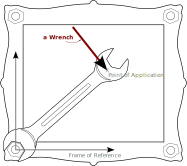
\includegraphics[width=8cm]{./figures/the_wrench.pdf}
\caption{\label{fig:wrench}\textbf{Wrench notation.} A Wrench is a combined vector of force and moment, consisting of six elements, and requiring a point of application. Wrench vectors are depicted as arrows, yet in contrast to forces, their tip points towards the point of application (they can be moved around, adjusting the moment component; see text). Note that this figure is actually a 3D sketch, yet the limitations of a printed PhD thesis prohibit illustration beyond the paper plane projection.}
\end{figure}


Any modern scripting language used to solve inverse dynamic questions can easily work on six element arrays/vectors instead of three-dimensional ones.
A mathematical shorthand for writing wrenches are square brackets and a semicolon indicating that the (column vector) components are concatenated (to form a longer column vector):
\[\vec{W} = \left[ \vec{F}; \vec{M} \right]\]

\begin{figure}[p]
\centering
\includegraphics[width=12cm]{./figures/slamming_wrench.pdf}
\caption{\label{fig:slamming_wrench}\textbf{The door slamming experiment in wrench notation (see text).} Point \(\vec{P}\) is the origin of the reference frame, \(\vec{r}_{\vec{PD}}\) is the position vector to the attack point \(\vec{D}\) of the wrench \(\vec{W}\).}
\end{figure}


\FloatBarrier
\subsection{Balance of Wrenches}
\label{sec:orgdcc1aac}
As with force and moment, we can equate a dynamic wrench to external wrenches in the calculation of a ``balance of wrenches''.
This can be achieved by, again, vertically concatenating force and moment balances.


For one, we get a ``dynamic wrench'' on the left hand side of the balance.
Plugging in the non-zero part of equations \eqref{eqn:force} and \eqref{eqn:moment} from above, we get an expression for what can be referred to as the \textbf{dynamic wrench} (defined at the \(\vec{COM}\)):
\begin{equation}\label{eqn:dynamic_wrench}
\vec{W}_{dyn} = \left[ m\frac{d^2\vec{x}}{dt^2}; I\frac{d^2\theta}{dt^2} \right]
\end{equation}

Wrenches can be added up, for example the dynamic wrench can be easily shifted (vector \(\vec{s}\)) to a different reference point, which does not require extra adjustment of the mass moment of inertia:
\begin{change}
\begin{equation}\label{eqn:shift_wrench}
\vec{W}_{dyn}^{*} = \vec{W}_{dyn} + [ \vec{0}; \vec{s} \times \underbrace{(m\frac{d^2\vec{x}}{dt^2})}_{\vec{F}} ]
\end{equation}
\end{change}



The \(\vec{x}\) and \(\theta\) in the dynamic wrench refer to the movement of the rigid body itself and are immediately derived from the object's kinematics.
The inertial properties \(m\) and \(I\) have to be measured or approximated separately.
The dynamic wrench expresses the \chng{rate of change} of momentum of an object.


On the other hand side of the equation, we have any \textbf{external wrenches} acting on the object.
The most important ones are the gravitational wrench, friction wrench, and the tip wrench (stay tuned).
\[\vec{W}_{\vec{g}} = \left[ m\vec{g}; 0 \right]\]
\[\vec{W}_{f} \approx \left[ 0; 0 \right]\]
\[\vec{W}_{\vec{tip}} = \left[ \vec{F}_{\vec{tip}}; \vec{M}_{\vec{tip}} \right]\]

We can sum up all external wrenches to get a total external wrench \(\vec{W}_{ext}\):
\begin{change}
\begin{equation}\label{eqn:external_wrench}
\vec{W}_{ext} = \sum\limits_{ext} \vec{W}_{i} = \vec{W}_{\vec{tip}} +\vec{W}_{\vec{g}}+\vec{W}_{f}+\ldots
\end{equation}
\end{change}

Any other known external forces and moments should be added in wrench form, keeping in mind that correct addition requires shift to the same reference point (usually the \(\vec{COM}\)).


Equations \eqref{eqn:dynamic_wrench} and \eqref{eqn:external_wrench} constitute the \textbf{Balance of Wrenches}:
\begin{equation}\label{eqn:balance_of_wrenches}
\vec{W}_{dyn} = \sum\limits_{ext} \vec{W}_{i}
\end{equation}


\newpage
In other words:
\begin{center}
The \chng{rate of} change of [linear;angular] momentum of a rigid body is equal to the sum of external wrenches acting on it.
\end{center}
\subsection{Reference Frames}
\label{sec:org5a5257c}

For simplicity, I ignored the issue of reference frames in all equations above.
Just like reference points, reference frames need to be well documented.
Transformation from one to another reference frame is possible by matrix multiplication with a transformation matrix.
It turns out that reference frames are not required for the calculations above: one can and should simply stay in the inertial reference frame.

If one, however, decides to venture into the reference frames (as the author did), be aware that fictitious forces add to the balance.
Interested readers may refer to a practical guide by the author \citep{Mielke2020wrenches}.
\subsection{Quaternions}
\label{sec:org2953b39}
\begin{figure}[b]
\centering
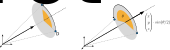
\includegraphics[width=16cm]{./figures/quaternions.pdf}
\caption{\label{fig:quaternion}\chng{\textbf{Spatial rotation with quaternions}. A point \(\vec{D}\) (blue, with gray dashed position vector) can be rotated by an angle \(\theta\) around an axis \((x; y; z)\) to position \(\vec{D}_{rot}\). The higher the rotation angle value (indicated by the orange area), the further the rotation. A quaternion (large black arrow) can encode both the axis and the angle in a 4D vector, in a manner which conveniently enables the execution of the rotation by simple vector multiplication.}}
\end{figure}

On top of the force/moment complexity comes the issue of quantifying rotation in space.
Angular momentum depends on angular acceleration \(\frac{d^2\theta}{dt^2}\), which is the second temporal derivative of ``angle''.
But getting that angle in 3D is not exactly trivial, and there are several complementary notations.


When we think about rotation in space, we might think about an axis and an angle \chng{(Fig. \ref{fig:quaternion})}.
And that is a good point to start.

\begin{center}
axis: \(\begin{pmatrix}x\\y\\z \end{pmatrix}\), angle: \(\theta\)
\end{center}

On the swinging door, the axis would be the line through the hinge points, and the angle could be measured as the radians separating open and closed state.
Ideally, one would want to combine axis and angle into a single object \(\vec{q}\), and it turns out that the following way is convenient \citep{Pennestri2010,Challis2020,Flashner2019}:
\begin{equation}\label{eqn:quaternion}
\begin{pmatrix}cos(\theta/2)\\x\cdot sin(\theta/2)\\y\cdot sin(\theta/2)\\z\cdot sin(\theta/2) \end{pmatrix} = \vec{q} = \begin{pmatrix}q_w\\q_x\\q_y\\q_z \end{pmatrix}
\end{equation}

There also exists a conjugate, \(\vec{q}^{-1}\):
\[\vec{q}^{-1} = (q_w, -q_x, -q_y, -q_z)\]


And this object \(\vec{q}\) allows for convenient spatial rotation, by almost-simple multiplication:
take any 3D point's position vector \(\vec{D}\) with 4D coordinates\footnote{The position vector \(\vec{D}\) is transferred to 4D space (formally necessary for multiplication with 4D quaternions) by simply appending a ``zero'' as the first element; the quaternion multiplication ensures that \(\vec{D}_{rot}\), though also 4D, always has a zero-valued first element, being effectively 3D.} (\(0, a, b, c\)).
This could be the door handle point from our example: after rotation, it will be \(\vec{D}_{rot}\), which can be calculated by:
\[\vec{D}_{rot} = \vec{q}\cdot \vec{D}\cdot \vec{q}^{-1}\]


The dot ``\(\cdot\)'' is just vector multiplication, and computational tools can handle this operation quickly and efficiently.
Better yet, one can stack quaternions by (non-commutatively) multiplying them:
\[ \vec{q}_2 \cdot \left( \vec{q}_1\cdot \vec{P}\cdot \vec{q}_1^{-1}\right) \cdot \vec{q}_2^{-1} = (\vec{q}_2\cdot \vec{q}_1) \vec{P} (\vec{q}_2\cdot \vec{q}_1)^{-1} \]

Working with time series of quaternions (\(\vec{q}(t)\), i.e. the angular position of an object changing over time), there is a formula for getting the angular velocity \(\frac{d\theta}{dt}\) from the time differences \(d\vec{q}/dt\) which fortunately even works with numeric differentials \(\frac{\Delta \vec{q}}{\Delta t}\) of real measurements \citep{Baker1999}.
\[\frac{d\theta}{dt} = 2 \frac{\Delta \vec{q}}{\Delta t} \cdot \vec{q}^{-1} \]

A quaternion variant for the Kabsch algorithm exists \citep{Kabsch1976,Lawrence2019,Kneller1991}.
This algorithm is useful to find the rotational difference between rigid bodies, including the change of rotation of a rigid body between two measurement times or the position of a segment relative to another.


Quaternion operations are usually included as functions in common quaternion toolboxes (for example in \href{https://www.mathworks.com/discovery/quaternion.html}{Matlab}, \href{https://cran.r-project.org/web/packages/onion/onion.pdf}{R}, and \href{https://pypi.org/project/numpy-quaternion}{Python}).
And toolboxes also provide the capability of conversion to other notations of spatial rotation (Euler- or Tait-Bryan angles, Rotation Matrices).


Just like with wrenches, quaternions cause discomfort to untrained analysts because they seemingly leave the familiar space of 3D geometry.
However, if one simply accepts that maths can handle 4D or 6D problems, the reward is computational convenience.
Superposition and the generation of temporal derivatives are readily available.
Quaternions also avoid some of the pitfalls of the alternative methods (gimbal lock problem, order dependence).
They have an intuitive geometric interpretation through the axis-angle-analogy.
And if anatomically relevant axes are required for communication, they can easily be transformed to such.

This does not imply that inverse dynamic calculations are impossible with Euler Angles.
Yet in most applications, quaternions are mathematically elegant and efficient.

\FloatBarrier
\section{Dynamics: Application}
\label{sec:org979aa90}

\subsection{Generic Approach}
\label{sec:orgb4239cb}
The theoretical considerations above assemble several technical advantages which are worth summarizing.
\begin{itemize}
\item The Balance of Wrenches, equation \eqref{eqn:balance_of_wrenches}, can be calculated entirely in the inertial reference frame, without repeated switch to joint coordinate systems (and return).
\item Wrenches can easily be moved to other reference points via equation \eqref{eqn:shift_wrench}.
\item A convenient point to calculate the balance of wrenches is the center of mass (\(\vec{COM}\)); rotation about that point is an expression of spin angular momentum (an intrinsic property) and most components simplify (e.g. gravitational wrench \(\vec{W}_{\vec{g}}\), dynamic wrench \(\vec{W}_{dyn}\)).
\item Expressing rotational motion by quaternions avoids issues of other methods; favorable features are linear superposition and direct derivative calculation.
\end{itemize}

These favorable technical properties have not gone unnoticed \citep{Dumas2004,Dumas2007}.
Dumas et al. (2004) presented a numeric procedure to perform segment-wise balance of wrenches \citep[equation 15 in][]{Dumas2004}.
This enables the complete solution of inverse dynamic problems with a single, easy to apply numeric formula.
Dumas \emph{et al.} have provided and since then improved an implementation of their procedure in Matlab \citep{DumasMatlab}.


The sceptical author of this thesis has reproduced that procedure in Python, both numerically and analytically \citep{Mielke2021id}.
\subsection{Algorithm}
\label{sec:orgf8cdb26}
With wrenches, quaternions, or the numerical formula at hand, one can compute the Balance of Wrenches for a single segment.
Limb segments are usually arranged in a chain, e.g. a human leg consists of the thigh, a lower leg, a foot, and toes.
However, there is an issue.
The inertial wrenches (gravitational wrench, friction, \ldots{}) are known; the dynamic wrench is measured from kinematics and inertials; yet connecting wrenches are usually unknown: each segment (e.g. the thigh) receives an unknown wrench input from all adjacent segments (e.g. the pelvis and the lower leg).

There is one exception: the distal-most segment which has ground contact.
Instrumented runways can contain force plates to measure contact forces and moments at the contact of the distal limb on the ground.
Force plates usually generate electronic read-outs from directional, pressure sensitive piezoelectric crystals.
By calibrating the plate, one can convert a voltage profile to forces, moments, and a contact point, all of which are changing over time.


Hence, the practical strategy \citep{Robertson2013,Lynch2017,Dumas2004} is to start at the most distal limb segment (e.g. the foot-toe or hoof complex), and measure its movement and ground contact wrench.
In that situation, all wrenches in the balance are known, except the wrench at the proximal joint (human foot example: the ankle wrench).
The external wrench at the ground contact point, in the balance calculation of the segment which is in ground contact, is also called the tip wrench; trivially, it is zero if the distal segment is lifted off the ground.
Note that the read-out of a force plate gives a contact point, which is not the \(\vec{COM}\), so the wrench can be taken at contact point and must then be shifted.
One can calculate the balance of wrenches by subtracting all external wrenches (ground contact wrench, gravitational wrench, proximal joint wrench, \ldots{}; all shifted to the \(\vec{COM}\) as the common reference point) from the dynamic wrench of the segment (measured linear and angular movement, also with respect to the \(\vec{COM}\)).
Exactly one of the external wrenches is unknown, the one on the proximal joint; we can solve for it (careful with reference points: the calculation comes out at the \(\vec{COM}\)).
The proximal joint wrench is shifted to the proximal joint position, its natural ``point of attack''\footnote{This series of shifts should have illustrated why the wrench is a useful construct: computational rigor can make sure that the reference points are respected.}.
Inverted in sign (Newton's \(n^{th}\) law), the joint wrench becomes the tip wrench of the proximally adjacent segment and adds to the balance of wrenches of that segment (Fig. \ref{fig:wrenchbalance}).
There, the procedure is repeated.

\begin{figure}[p]
\centering
\includegraphics[width=8cm]{./figures/wrench_balance.pdf}
\caption{\label{fig:wrenchbalance}\textbf{Wrench balance of a piglet femur (sketch)}, as it can be computed for each segment from distal to proximal. The tip wrench (\(\vec{W}_{\vec{tip}}\), at the distal joint) is the input from the distal adjacent segment or from ground contact. Dynamic wrench (\(\vec{W}_{dyn}\), at the center of mass/\(\vec{COM}\)) is calculated from kinematics. Gravitational wrench (\(\vec{W}_{\vec{g}}\), at \(\vec{COM}\)) is known by the mass of the segment. These wrenches allow to calculate the joint wrench (\(\vec{W}_{joint}\), at the proximal joint), which is the tip wrench input for the proximal adjacent segment. All calculations can be performed in the inertial coordinate system (\(ICS\), i.e. the inertial reference frame).}
\end{figure}
\subsection{Inertial Properties}
\label{sec:orga26581e}
The procedure is quite trivial to implement, however the measurement uncertainty for all the involved quantities is not homogeneous.
Whereas force plates and spatial coordinates can be accurately measured in a calibrated lab reference frame, the \textbf{inertial properties} of each segment require rough measurements and approximation.
The relevant inertial properties are mass \(m\), center of mass \(\vec{COM}\), and mass moment of inertia \(I\).
This justifies a closer look at them.


There are several ways to retrieve inertial properties.
The classical method requires a dissection of the segment; this can be a precise anatomical disarticulation or straight-cut slicing of a frozen specimen.
In the case of our slamming door, one would take the door off the hinge.
The segment mass is then measured on a simple scale.
Center of mass could be derived from a classical pendulum experiment (Fig. \ref{fig:door_inertials}): hang an object from a thread, measure oscillation period, apply \(T=2\pi\sqrt{\frac{l}{\vec{g}}}\) solved for effective length \(l\), repeat the procedure with the object hung along a different axis.
A common simplification is to express the position of the \(\vec{COM}\) as a fraction of the segment length, inaccurately assuming that it lies on the segment long axis.
Anatomical landmark references are required to transform the relative \(\vec{COM}\) position into the lab reference frame.
Finally, the classical method to determine mass moment of inertia is by using a trifilar pendulum \citep{Schedlinski2001,Korr1962,Wells1987}.

The so-retrieved measurements are filled in to the algorithm outlined above.


\begin{figure}[p]
\centering
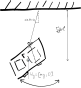
\includegraphics[width=10cm]{./figures/door_inertials.pdf}
\caption{\label{fig:door_inertials}\textbf{Measuring inertial properties of the slamming door:} the center of mass.}
\end{figure}


Measurement uncertainty of the inertial properties is not determined by the accuracy of the measurement instruments.
This is where the ``slamming door'' analogy fails, because a door is actually rigid.
The pendulum methods above yield numerically accurate results.
However, the dissected limb is only a limited representation of the segment \emph{in vivo}, for several reasons.

A first issue is the choice of a disarticulation cutting surface: which mass particles are assigned to which segment?
This choice affects mass, but also \(\vec{COM}\) and mass moment of inertia, and because cuts are generally further away from the \(\vec{COM}\), this effect matters.

Second, muscles (as a complex composition of fiber bundles and fibers) deform, shift and slide past each other during contraction and movement \citep{Bol2013}.
Their cross section and fibre distribution can change on non-isometric movements.
Gravity pulls soft tissue into a direction \citep{Hansraj2022} which might be different \emph{in vivo} and on the preserved configuration of the limb.
Zeugopodial and autopodial segments often include multiple bones which might experience a shift in their relative position during a stride cycle.
All this reduces congruence of the preserved, measured body part and the \emph{in vivo} situation: mass is constant, yet the \(\vec{COM}\) of a segment is not stable during locomotion, and the mass moment of inertia tensor will most certainly vary during the process.

Third, there might be shrinkage and tissue loss during the preservation of the specimen.
Formol, ethanol, or temperature are typical agents used as a fixative; any fixative has its effect on soft tissue \citep{Buytaert2014,Pech1987}.
This issue can putatively change all inertials properties of the sample.

Fourth, 3D volumetric imaging (e.g. CT scans) could be an option to replace the measurements above, yet such scans do not solve all of the other issues, and instead come with their own set of problems and limitations (topic of the next chapter).



The implications of these conceptual issues will be discussed in detail in the next chapter.
Yet note already that these four effects violate an assumption above: inertial properties are hard to determine, and the velocity product terms in the balance of forces are non-negligible because the mass distribution is not constant.


\clearpage
\section{Summary}
\label{sec:org931c4c7}
This chapter serves as a brief overview of the basic methodology of inverse dynamics.
This method exploits the fundamental physical phenomenon of conservation of momentum to model and infer the reasons for movement of systems of more or less rigid bodies.
I outlined the general algorithm, and documented one specific procedure applicable to inverse dynamic measurements of quadruped, terrestrial locomotion.


In particular, the Wrench-Quaternion method \citep{Dumas2004} has proven useful for joining kinematics and force measurements for dynamic calculation.
The reason is computational convenience.
Wrenches are the conceptual link of forces and moments, and they allow convenient computer implementations.
Quaternions have favorable properties to calculate spatial rotation in the context of rigid body motion (superposition, singularity avoidance, transformability).
This establishes the conceptual framework to perform the relevant calculations of the conventional algorithm, which involves starting at the distal segments where external forces are known (e.g. ground contact) and processing the calculation towards the torso of the animal.


A crucial simplification of that procedure is that we treat body segments of animals as rigid bodies, which they are not.
By \emph{post mortem} fixation and dissection, or by \chng{digital volumetric segmentation}, segments can be separated and their inertial properties measured.
The accuracy of these methods will be the topic of the next chapter.
